\documentclass[10 pt,usenames,dvipsnames, oneside]{article}
\usepackage{../../../modelo-ensino-medio}


\begin{document}

\begin{center}
  \begin{minipage}[l]{3cm}
\includegraphics[width=2cm]{logo}    
\end{minipage}\hfill
\begin{minipage}[r]{.8\textwidth}
 {\Large \scshape Atividade: Imaginando gráficos}  
\end{minipage}
\end{center}
\vspace{.2cm}

\ifdefined\prof
\begin{objetivos}
\item \textbf{LAF1} Compreender função como uma relação de dependência entre duas variáveis, as ideias de domínio, contradomínio e imagem, e suas representações algébricas e gráficas e utilizá-las para analisar, interpretar e resolver problemas em contextos diversos, inclusive fenômenos naturais, sociais e de outras áreas.
\end{objetivos}

\begin{goals}
\begin{enumerate}

\item[OE1] Reconhecer o comportamento crescente e decrescente de funções a partir de suas representações dadas. Sugere-se, associar esse comportamento a situações cotidianas.

\end{enumerate}

\tcblower

\begin{itemize}
\item Não existe resposta única para cada item. Certifique-se de que seus estudantes tenham argumentos consistentes sobre as suas escolhas. Você pode sugerir que eles compartilhem entre si os seus argumentos.

\item É fundamental definir o que representa cada eixo, por exemplo, no item (I), se consideramos o tempo no eixo horizontal e a intensidade sonora no vertical, somente os gráficos (e) e (h) consideram o silêncio inicial, no entanto o gráfico (h) não leva em conta que “\textit{rapidamente} todos estavam aplaudindo e se manifestando”{} e ainda há diminuição na intensidade sonora. Portanto, o gráfico (e) é o mais adequado. Agora, caso coloquemos no eixo horizontal a quantidade pessoas aplaudindo, os mais adequados são os gráficos (a) ou (d), eles passam pela origem e são crescentes.
\end{itemize}

\end{goals}

\bigskip
\begin{center}
{\large \scshape Atividade}
\end{center}
\fi

Associe cada uma das situações apresentadas a seguir a um dos gráficos dados abaixo. Explique sua escolha e escreva, em cada um dos eixos, o que eles representam.
\begin{figure}[H]
\centering

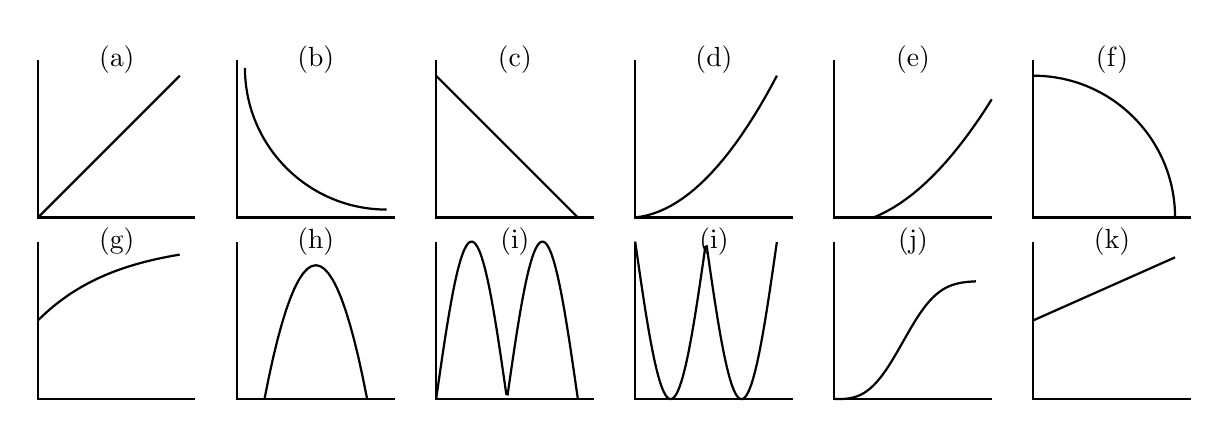
\begin{tikzpicture}
\node [matrix, column sep =.5cm] at (0,0)   {\draw[thick](0,2)--(0,0)--(2,0);\draw(1,2)node{(a)};\draw[thick](0,0)--(1.8,1.8);  &  \draw[thick](0,2)--(0,0)--(2,0);\draw(1,2)node{(b)};\draw[thick](0.1,1.9) arc(180:270:1.8);&\draw[thick](0,2)--(0,0)--(2,0);\draw(1,2)node{(c)};\draw[domain= 0:1.8,thick] plot(\x,1.8-\x); &\draw[thick](0,2)--(0,0)--(2,0);\draw(1,2)node{(d)};\draw[domain= 0:1.8,thick] plot(\x,.5*\x^2+.1*\x);&\draw[thick](0,2)--(0,0)--(2,0);\draw(1,2)node{(e)};\draw[domain= 0:2,thick] plot(\x,{max(0,.4*\x^2-.1)});&\draw[thick](0,2)--(0,0)--(2,0);\draw(1,2)node{(f)};\draw[thick](1.8,0) arc(0:90:1.8);\\  \draw[thick](0,2)--(0,0)--(2,0);\draw(1,2)node{(g)};\draw[domain=0:1.8,thick, samples=100]plot(\x, {2-exp(-\x)});& \draw[thick](0,2)--(0,0)--(2,0);\draw(1,2)node{(h)};\draw[domain=0.35:1.65,thick]plot(\x,{1.7-4*(1-\x)^2});& \draw[thick](0,2)--(0,0)--(2,0);\draw(1,2)node{(i)};\draw[domain=0:1.8, samples=100,thick]plot(\x,{abs(2*sin(200*\x))});&\draw[thick](0,2)--(0,0)--(2,0);\draw(1,2)node{(i)};\draw[domain=0:1.8, samples=100,thick]plot(\x,{2-(abs(2*sin(200*\x))});&\draw[thick](0,2)--(0,0)--(2,0);\draw(1,2)node{(j)};\draw[domain=0:1.8, samples=100,thick]plot(\x,{1.5-1.5*exp(-\x^3)});&       \draw[thick](0,2)--(0,0)--(2,0);\draw(1,2)node{(k)};\draw[thick](0,1)--(1.8,1.8);\\};
\end{tikzpicture}
\end{figure}

\begin{enumerate}[label=($\Roman*$)]
\item Após um concerto, houve um grande silêncio. Então uma pessoa na platéia começou a aplaudir. Gradualmente, as pessoas à sua volta também começaram a apludir de forma que rapidamente todos estavam aplaudindo.

\item Se o preço cobrado pelo ingresso de um cinema for muito baixo, seu prorietário irá perder dinheiro. Por outro lado, se o valor cobrado for muito alto, poucas pessoas irão pagar e novamente o proprietário vai perder dinheiro. Um cinema deve portanto cobrar um preço moderado por seu ingresso de forma que seja lucrativo.

\item Preços estão agora subindo mais lentamente do que em qualquer época nos últimos cinco anos.
\end{enumerate}
\begin{itemize}
\item {} 
Adaptado do artigo \emph{Michal Ayalon \& Anne Watson \& Steve Lerman (2015). Progression Towards Functions: Students’ Performance on Three Tasks About Variables from Grades 7 to 12.}
\end{itemize}

\ifdefined\prof
\begin{solucao}
\begin{enumerate}[label=($\Roman*$)]
\item (e) eixo horizontal, eixo vertical: intensidade sonora.

\item (h) eixo horizontal: número de clientes, eixo vertical: lucro.

\item (k) eixo horizontal: tempo, eixo vertical: preço

\end{enumerate}
\end{solucao}
\fi

\end{document}